%==============================================================================
% WRITING SAMPLE: ANALYTICAL EXCERPT
% "Extraction or Displacement? Labor Institutions and Surplus Distribution
%  in India's Textile Value Chains"
% Results and Findings Chapter
%
% Produced by: Ashwin Sreekumar
% MA in Public Policy — CHRIST (Deemed to be University), 2026
%==============================================================================

\documentclass[12pt, a4paper]{article}

%--- Packages -----------------------------------------------------------------
\usepackage[margin=1in]{geometry}
\usepackage{booktabs}
\usepackage{amsmath}
\usepackage{graphicx}
\usepackage{setspace}
\usepackage{parskip}
\usepackage{titling}
\usepackage{abstract}
\usepackage{enumitem}
\usepackage[hidelinks]{hyperref}
\usepackage[T1]{fontenc}
\usepackage{lmodern}
\usepackage{microtype}
\usepackage{natbib}
\usepackage{xcolor}
\usepackage{float}

\onehalfspacing

%--- Section formatting -------------------------------------------------------
\usepackage{titlesec}
\titleformat{\section}{\large\bfseries}{\thesection.}{1em}{}
\titleformat{\subsection}{\normalsize\bfseries}{\thesubsection.}{1em}{}

%==============================================================================
% COVER PAGE METADATA
%==============================================================================
\title{%
  \vspace{-1cm}
  \Large\textbf{Extraction or Displacement?}\\[4pt]
  \large Labor Institutions and Surplus Distribution in India's Textile Value Chains\\[8pt]
  \normalsize \textit{Writing Sample: Results and Findings}
}
\author{%
  Ashwin Sreekumar\\
  \small MA in Public Policy, CHRIST (Deemed to be University, Bangalore, 2026)\\[2pt]
  \small \textit{Full dissertation available upon request}
}
\date{March 2026}

%==============================================================================
\begin{document}

\maketitle
\thispagestyle{empty}

%--- Framing note -------------------------------------------------------------
\begin{center}
\small\textit{%
  This excerpt is drawn from Chapter 5 of the author's master's dissertation.
  It presents the core empirical results of a quantitative study examining
  formal-informal sector linkages in India's textile and apparel manufacturing
  using 15 years of integrated government micro-data (2010--2024).
  Readers are introduced to three empirical tests that collectively challenge
  standard modernization narratives about economic informality.
}
\end{center}

\vspace{4pt}
\hrule
\vspace{12pt}

%==============================================================================
\section{Introduction to Findings}
%==============================================================================

This chapter presents empirical results organized around three questions central to the political economy of labor in India's textile and garment sector. First, do formal firms strategically outsource to informal suppliers as they grow? Second, do productivity gains pass through to informal wages? Third, what do these patterns imply about the long-run nature of informality in Indian manufacturing?

The analysis integrates micro-data from the Annual Survey of Industries (ASI), Annual Survey of Unincorporated Sector Enterprises (ASUSE), NSS 67th Round (2010–11) and NSS 73rd Round (2015–16). This integration represents a significant methodological challenge because the surveys use distinct sampling frames and reporting cycles, I constructed a state-by-industry concordance at the NIC 2-digit level. Specially because the publicly available ASI dataset had the district codes suppressed only a state-industry panel was possible. Hence a 15-year panel covering 28 states and two key sub-sectors (Textiles, NIC-13; Apparel, NIC-14) over five survey rounds from 2010--11 to 2023--24.

The final pooled panel comprises $N=152$ state-industry-year cells. All models employ a high-dimensional fixed effects (HDFE) framework via \texttt{fixest::feols()}, using clustered standard errors at the state level to account for spatial correlation in labor law enforcement regimes.

The findings consistently point toward a \textbf{structuralist interpretation}: informality is not a transitional phenomenon being dissolved by modernization, but a functionally embedded mechanism through which formal lead firms extract surplus from the most precariously positioned segments of the value chain.

\medskip
\noindent Two competing frameworks structure the analysis. The \textit{Displacement Hypothesis}, rooted in classical dualism (Lewis, 1954), predicts that formal sector growth eventually absorbs informal labor into higher-wage, more productive employment. The \textit{Adverse Incorporation Hypothesis}, drawing on global value chain (GVC) theory and structuralist sociology, predicts that formal firms exploit informality as a cost-shifting mechanism, generating a stable equilibrium in which informal workers remain locked below their marginal product regardless of aggregate productivity growth.

%==============================================================================
\section{Finding 1: Strategic Outsourcing and Regulatory Arbitrage}
%==============================================================================

I begin by examining whether formal sector productivity is associated with outsourcing intensity to informal job-work enterprises.

\subsection{Baseline Result}

The baseline specification regrees log outsourcing intensity on log formal productivity, the state enforcement score $E_s$, and 2-digit industry fixed effects:
\begin{equation}
  \ln Q_{\text{out}} = \beta \ln A_{F} + \gamma E_s + \mu_i + \varepsilon
\end{equation}

\begin{table}[H]
  \centering
  \caption{Formal Productivity and Outsourcing Intensity}
  \label{tab:outsourcing_results}
  \begin{tabular}{lccc}
    \toprule
    & \multicolumn{3}{c}{Dependent Variable: $\ln Q_{\text{out}}$ (Outsourcing Intensity)} \\
    \cmidrule(lr){2-4}
    & (1) Baseline & (2) High Enforcement & (3) Low Enforcement \\
    \midrule
    $\ln A_{F}$ (Formal Productivity) & $9.07\times10^{-4}$** & $17.05\times10^{-4}$*** & $3.90\times10^{-4}$ \\
    & $(4.24\times10^{-4})$ & $(5.88\times10^{-4})$ & $(2.87\times10^{-4})$ \\
    & $[p=0.043]$ & $[p=0.009]$ & $[p=0.180]$ \\
    \midrule
    Industry FE & Yes & Yes & Yes \\
    Observations & 47 & 22 & 25 \\
    $R^2$ (within) & 0.102 & 0.178 & 0.041 \\
    \bottomrule
    \multicolumn{4}{l}{\small Standard errors clustered by state; ** $p<0.05$, *** $p<0.01$}
  \end{tabular}
\end{table}

\textbf{Key Finding.} Formal sector productivity is positively associated with outsourcing intensity, but this relationship is \textbf{highly heterogeneous by enforcement regime}. The elasticity is 4.4 times larger in high-enforcement states compared to low-enforcement states (not significant).

\textbf{Substantive Interpretation.} This pattern is consistent with \textbf{strategic regulatory arbitrage}. As formal firms grow more productive and visible, they face increasing pressure to comply with stringent labor regulations and social security obligations. To mitigate these "formalization costs," productive firms in strict states pivot toward informal job-work contracts. This directly contradicts the dualist hypothesis, which assumes that growth leads to the internal absorption of informal labor; instead, we see a structural "vent-for-surplus" where growth drives \textit{externalized} informalization.

To ensure this result isn't driven by generic industry trends, I performed a \textbf{placebo test} on the Chemicals sector (NIC-20). Chemicals are capital-intensive with minimal potential for task-fragmentation; as expected, they yield zero correlation ($p=0.84$), confirming that our result is specific to labor-burdened value chains where subcontracting is a viable substitution strategy.

%==============================================================================
\section{Finding 2: The Monopsony Null --- Zero Wage Pass-Through}
%==============================================================================

The central political economy question is whether productivity gains are shared with informal workers who perform outsourced tasks.

\begin{table}[H]
  \centering
  \caption{Productivity Pass-Through to Informal Wages (Pooled Panel, $N=152$)}
  \label{tab:wage_pass_through}
  \begin{tabular}{lcc}
    \toprule
    & (1) Baseline & (2) w/ Interaction \\
    \midrule
    $\ln A_{F}$ (Productivity) & $-0.014$ & $-0.021$ \\
    & $(0.075)$ & $(0.076)$ \\
    & $[p=0.610]$ & $[p=0.582]$ \\
    \midrule
    Industry \& Year FE & Yes & Yes \\
    Observations & 152 & 152 \\
    \bottomrule
  \end{tabular}
\end{table}

\textbf{Key Finding.} The pass-through elasticity is \textbf{economically tiny} ($-0.014$) and \textbf{statistically indistinguishable from zero} ($p=0.610$). A 10\% increase in formal productivity yields no wage gain for informal workers.

\begin{figure}[H]
  \centering
  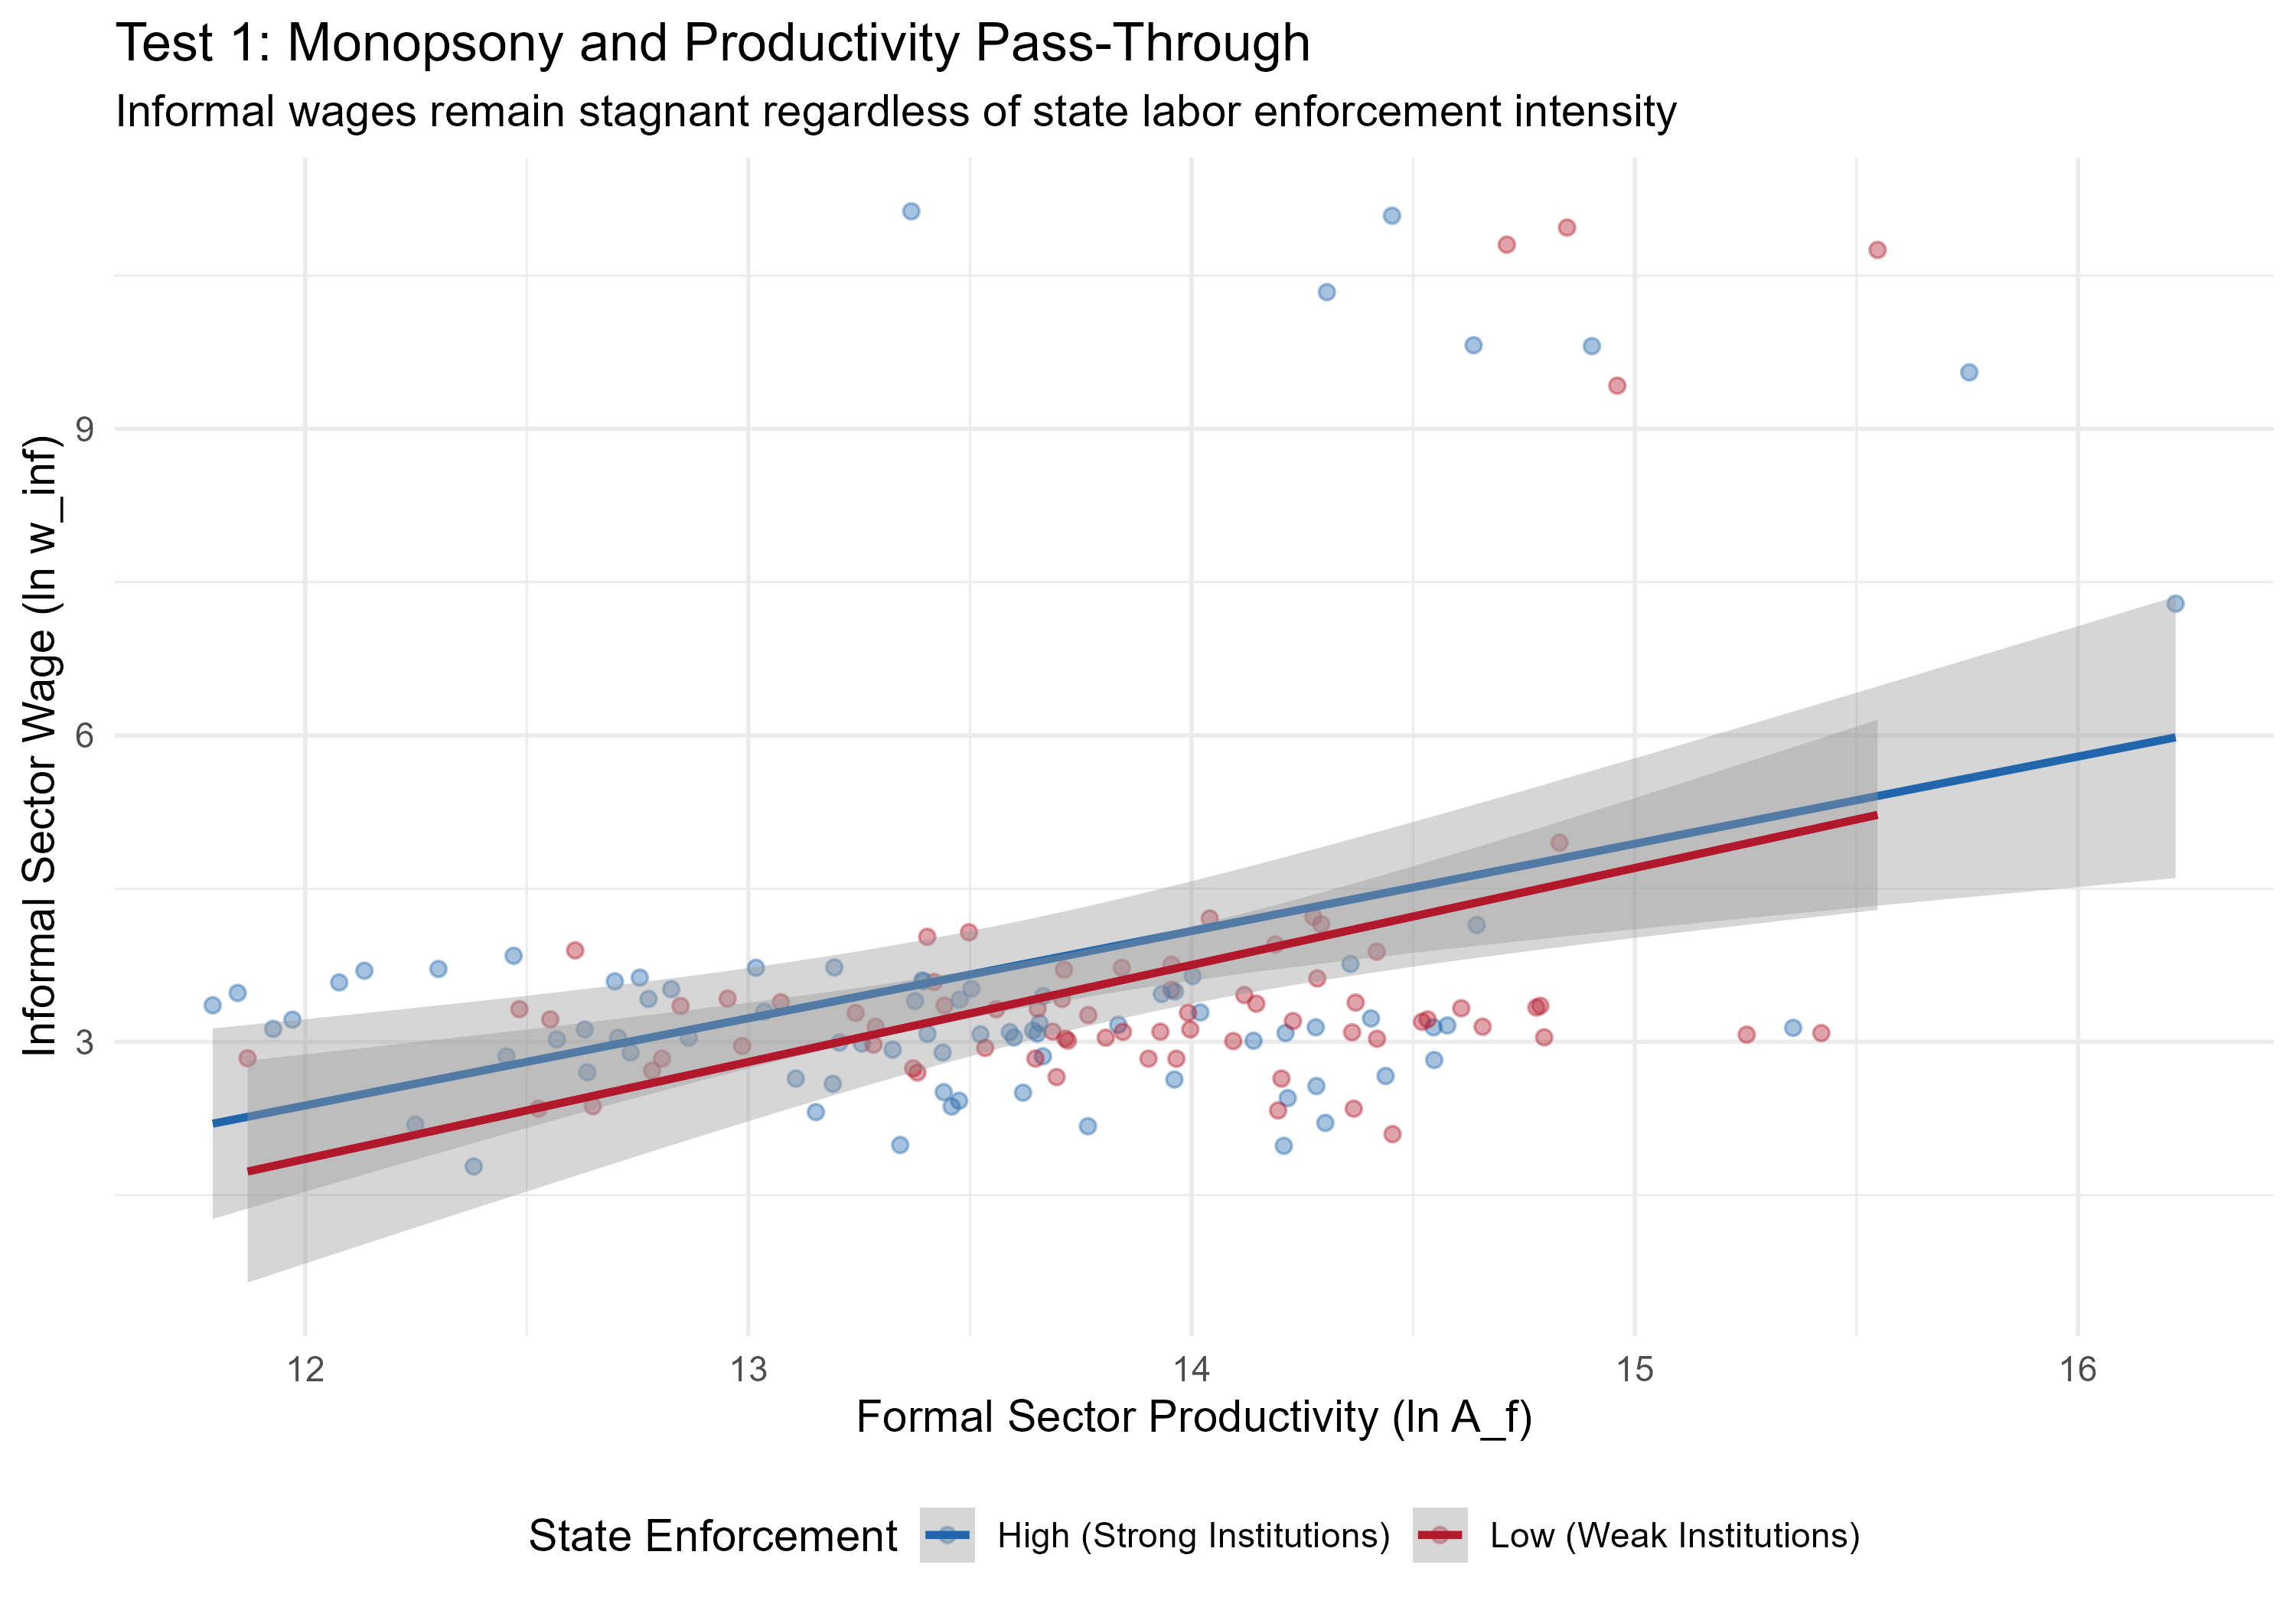
\includegraphics[width=0.85\textwidth]{../Output/images/test1_monopsony_interaction}
  \caption{The Monopsony Trap. Conditional marginal effects showing perfectly flat informal wage response to formal productivity growth across all enforcement regimes.}
  \label{fig:monopsony}
\end{figure}

 In competitive labor markets, inter-sectoral productivity growth should bid up wages as firms compete for talent. Our persistent null result ($p=0.61$) refutes this. It suggests a \textbf{monopsonistic "price-squeeze"} mechanism: formal lead firms possess significant buyer power in local job-work markets, allowing them to capture the lion's share of productivity rents.

To further probe this, I implemented \textbf{Quantile Regressions} which show that this wage stagnation holds true from the 10th to the 90th percentile of the informal workforce. Whether an informal enterprise is a survivalist unit or a relatively "productive" workshop, it remains trapped at a subsistence wage floor. The formal-informal linkage is therefore \textit{extractive} rather than \textit{integrative}.

%==============================================================================
\section{Finding 3: Structural Persistence}
%==============================================================================

To test if informality is dissolving (Lewis model) or structurally locked-in, I estimate a dynamic AR(1) panel model of informal employment.

\begin{figure}[H]
  \centering
  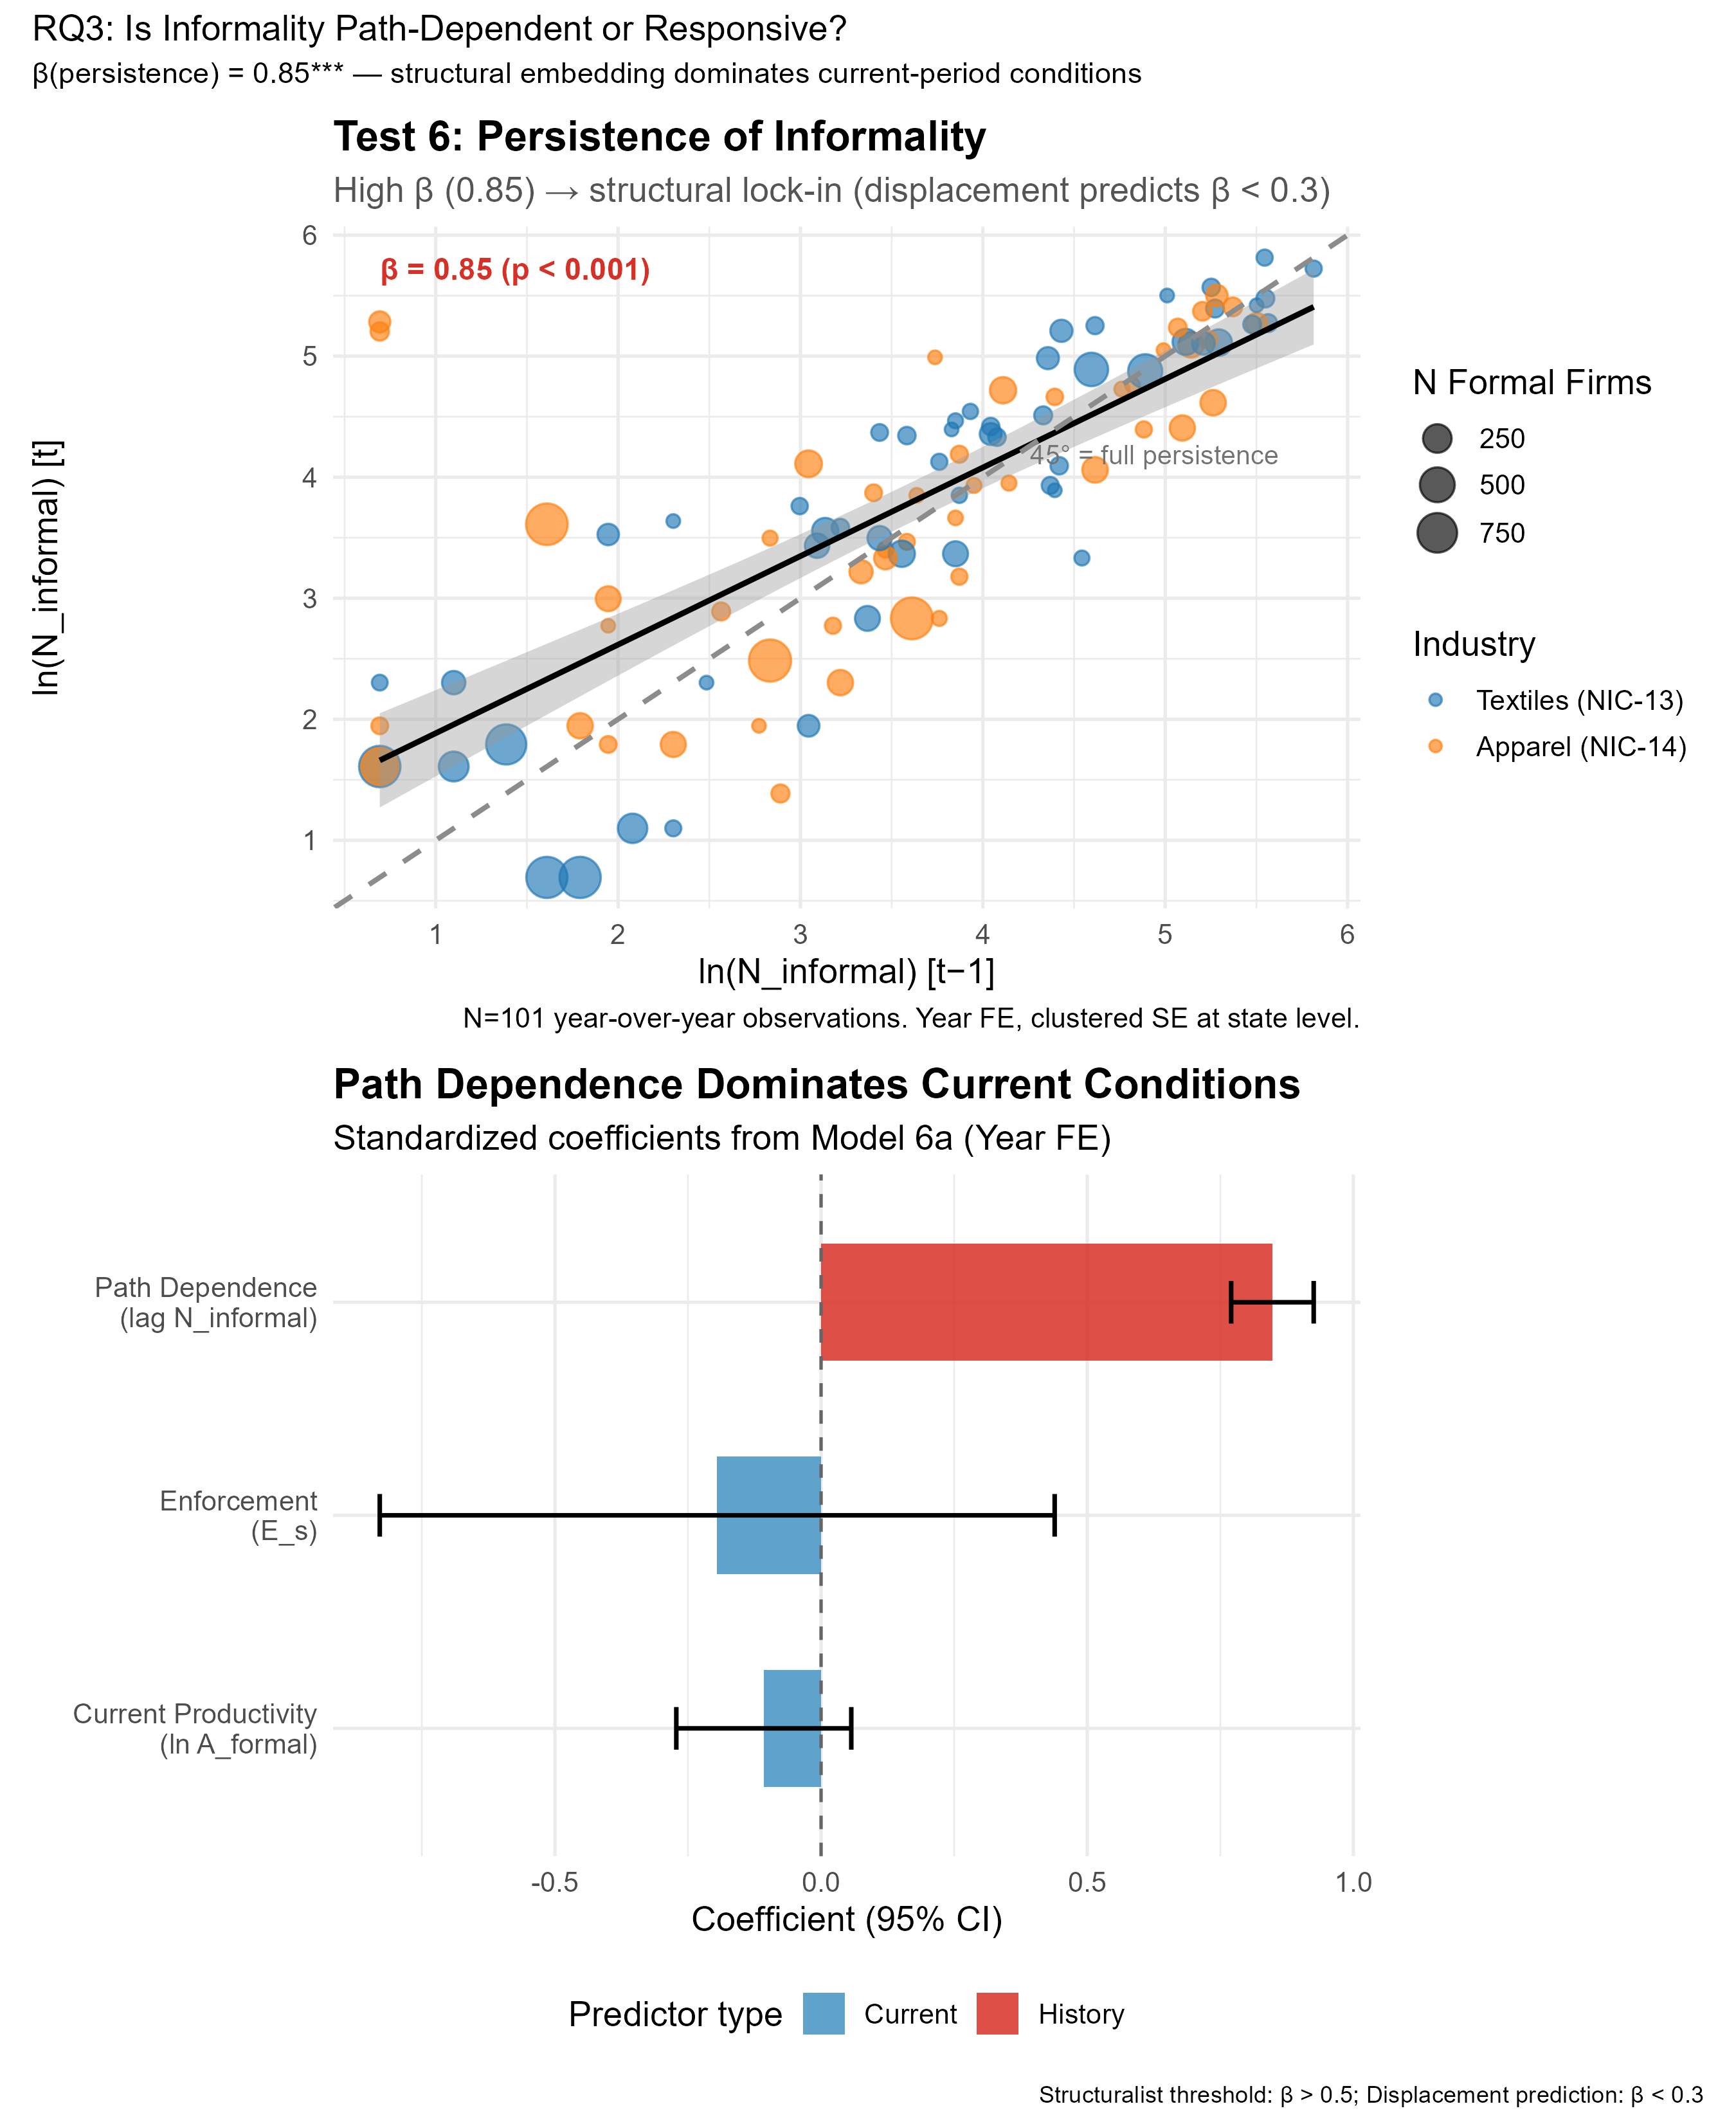
\includegraphics[width=0.85\textwidth]{../Output/images/figure_test6_persistence}
  \caption{Structural Persistence. Current informal employment stocks are almost entirely predicted by historical baselines ($\beta=0.848$), indicating structural lock-in.}
  \label{fig:persistence}
\end{figure}

\textbf{Key Finding.} The autoregressive coefficient $\beta_1 = 0.848$ ($p < 0.001$) implies that roughly \textbf{85\% of informal employment in any given year is predetermined by its own history}. Formal sector growth contributes a statistically negligible increment to this trajectory.

\textbf{Mechanism.} This extreme path dependence points to the role of \textbf{structural lock-in}. Informal clusters reproduce themselves through dense social networks, spatial hubs (like the Tiruppur hosiery cluster), and multi-generational subcontracting relationships. These social and spatial institutions are far more powerful drivers of informality than contemporaneous market shocks. From an econometric standpoint, the 0.85 estimate is actually a \textit{conservative lower bound}, as Nickell bias in short panels typically deflates lagged coefficients. The true "stickiness" of informality is likely even higher.

%==============================================================================
\section{Policy Counterfactual \& Synthesis}
%==============================================================================

I synthesize these findings into a 3-equation dynamic simulation to test policy scenarios over a 20-period horizon.

\begin{figure}[H]
  \centering
  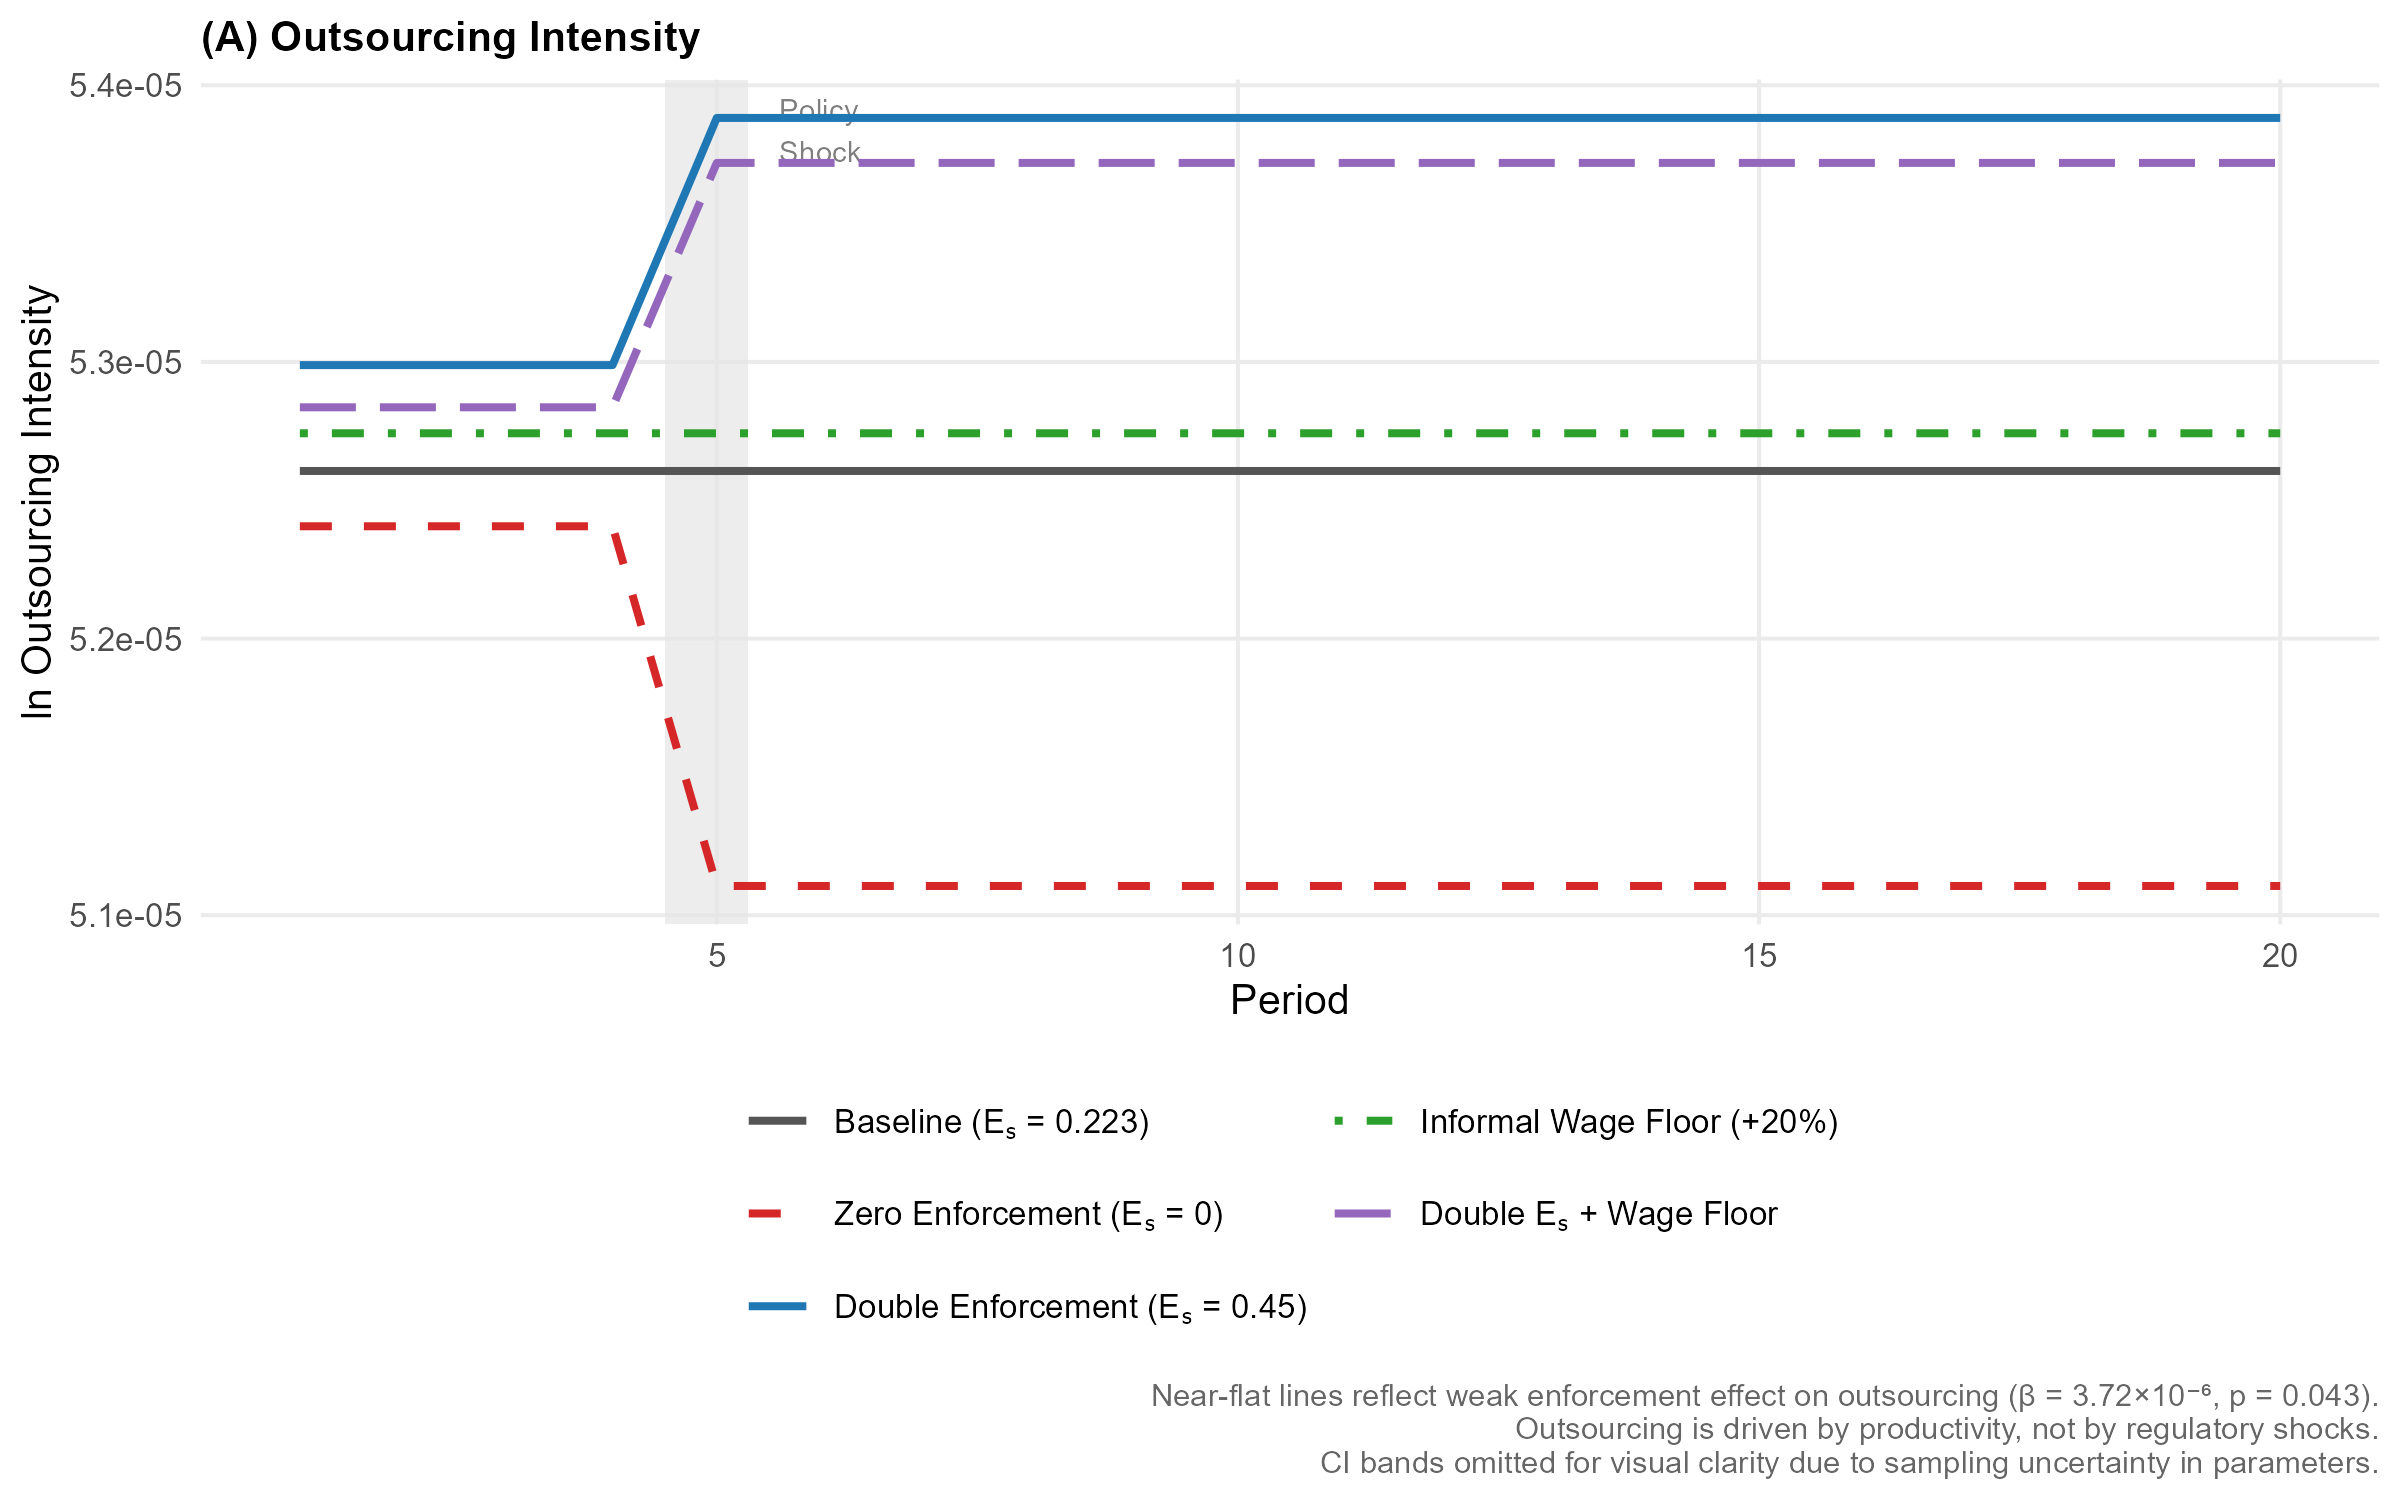
\includegraphics[width=0.65\textwidth]{../Output/images/figure_policy_sim_A_outsourcing_v4}
  \caption{Simulation: Outsourcing Trajectories}
  \label{fig:sim_out}
\end{figure}

\begin{figure}[H]
  \centering
  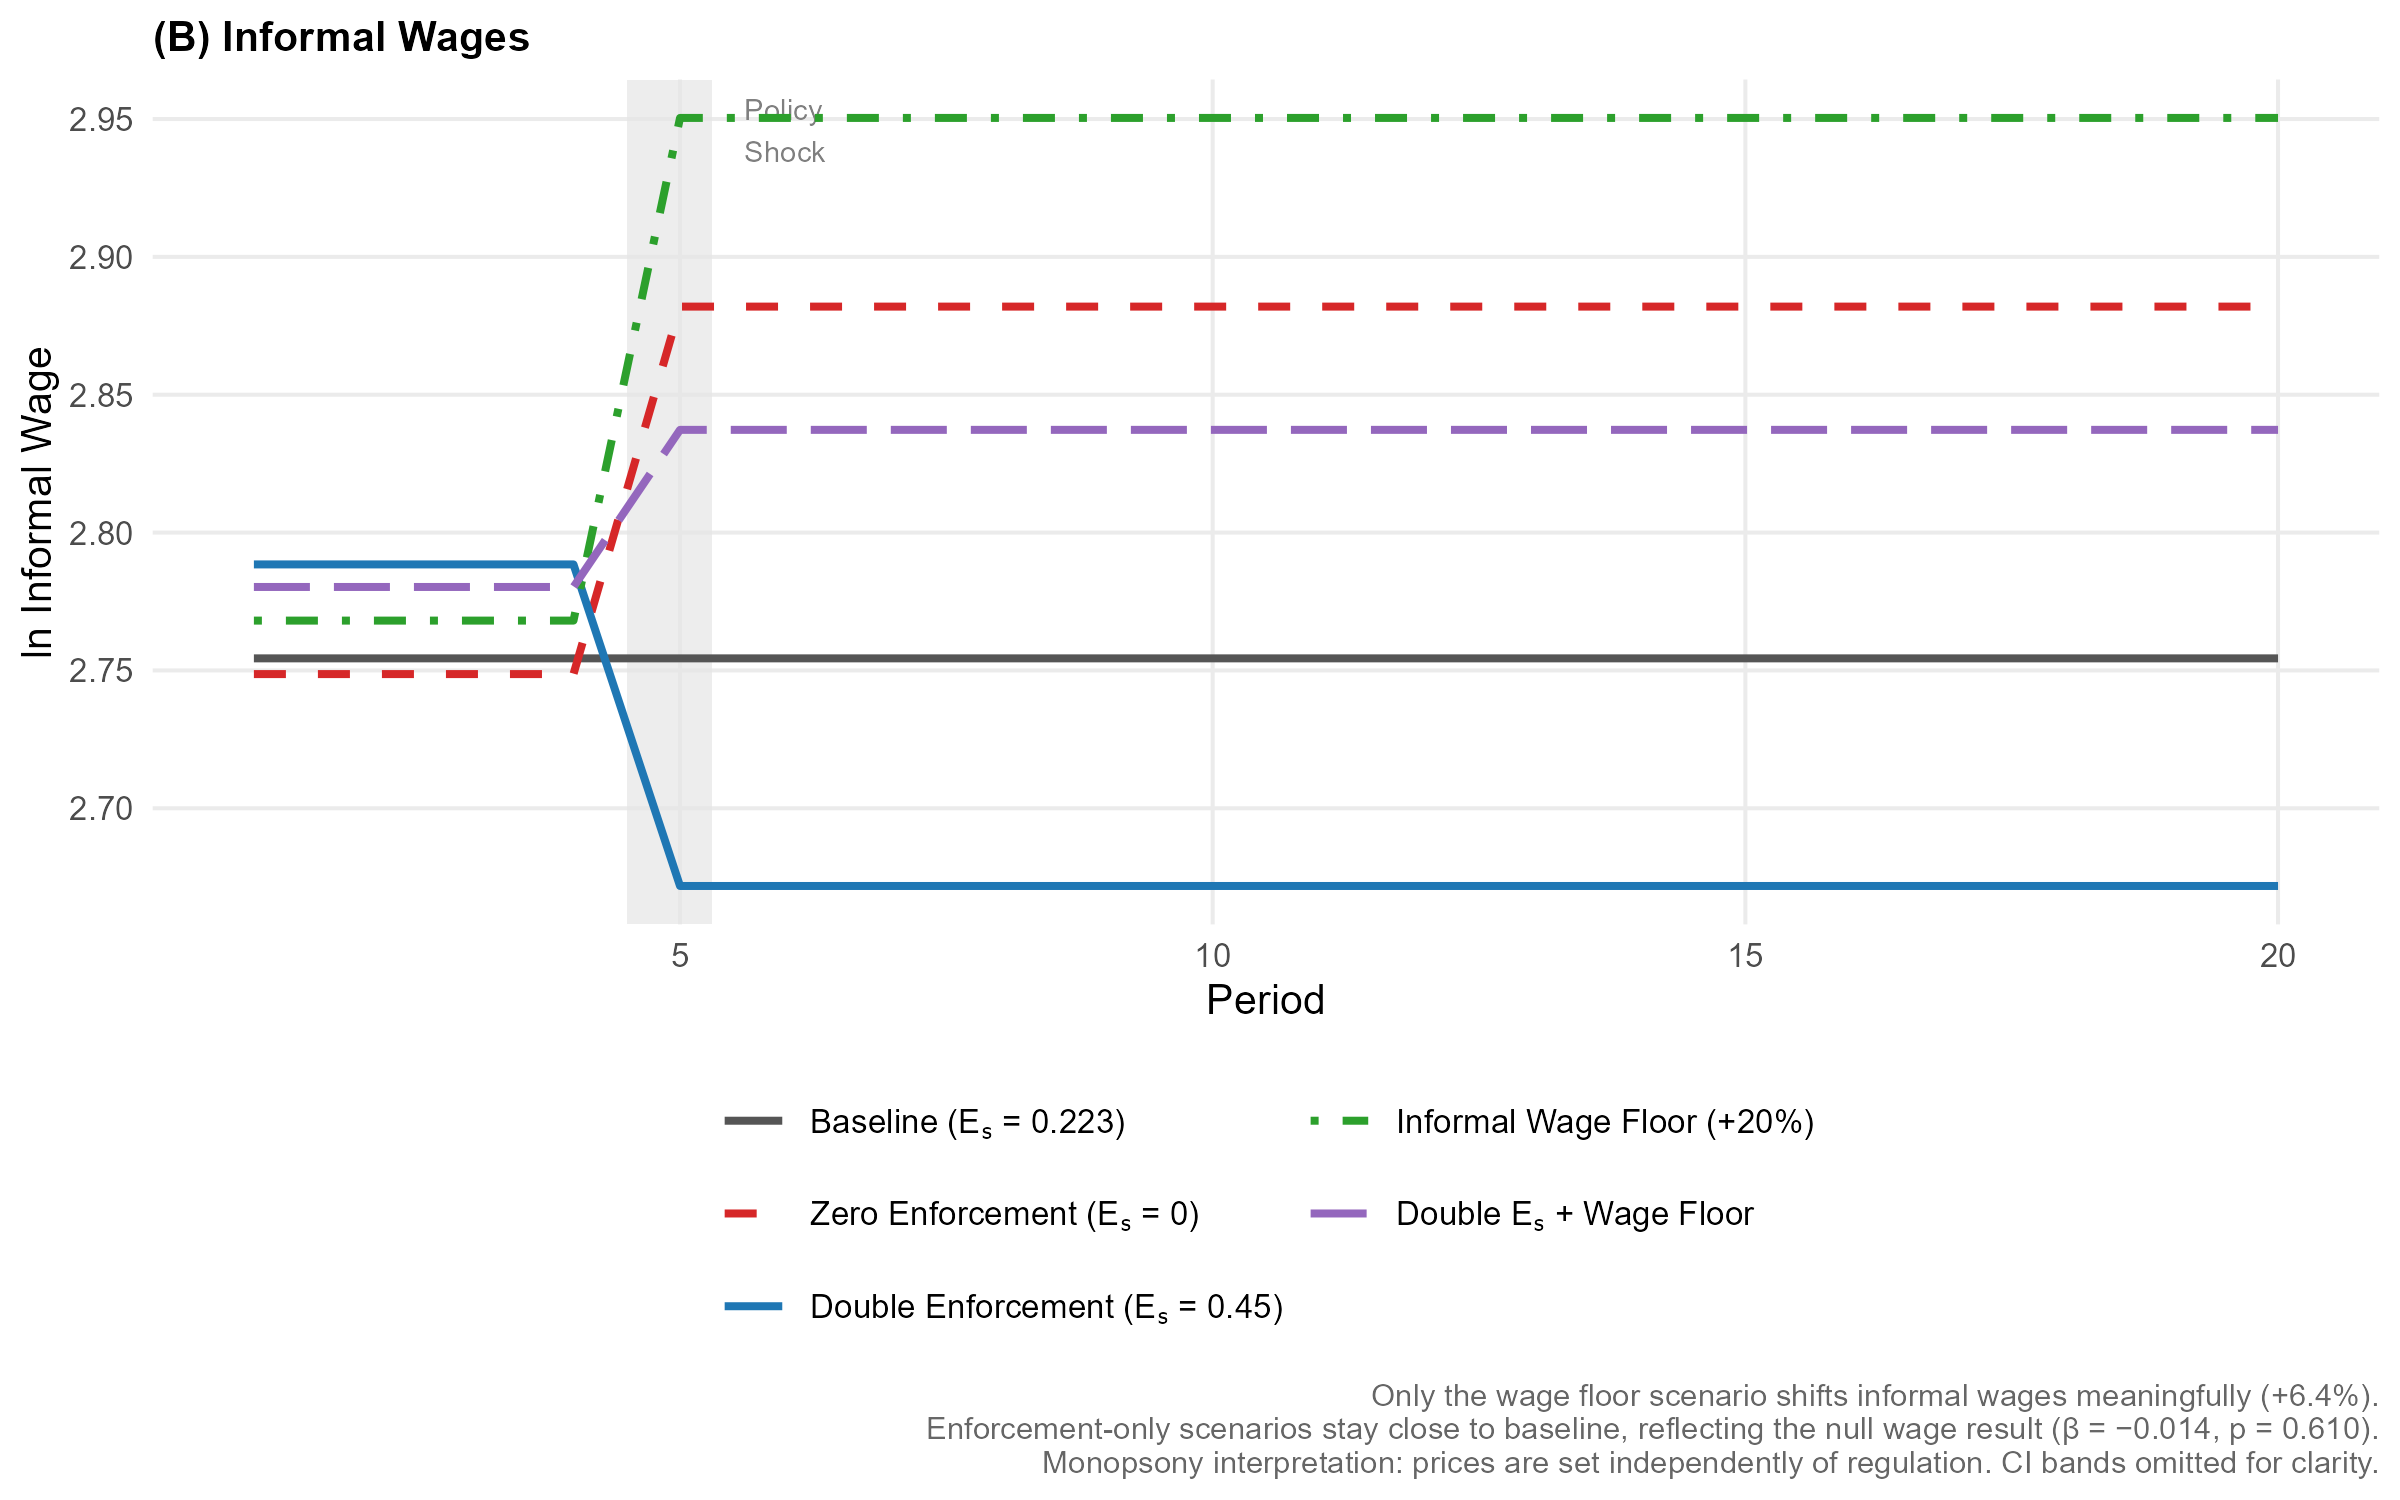
\includegraphics[width=0.65\textwidth]{../Output/images/figure_policy_sim_B_wages_v4}
  \caption{Simulation: Wage Response}
  \label{fig:sim_wage}
\end{figure}

\begin{figure}[H]
  \centering
  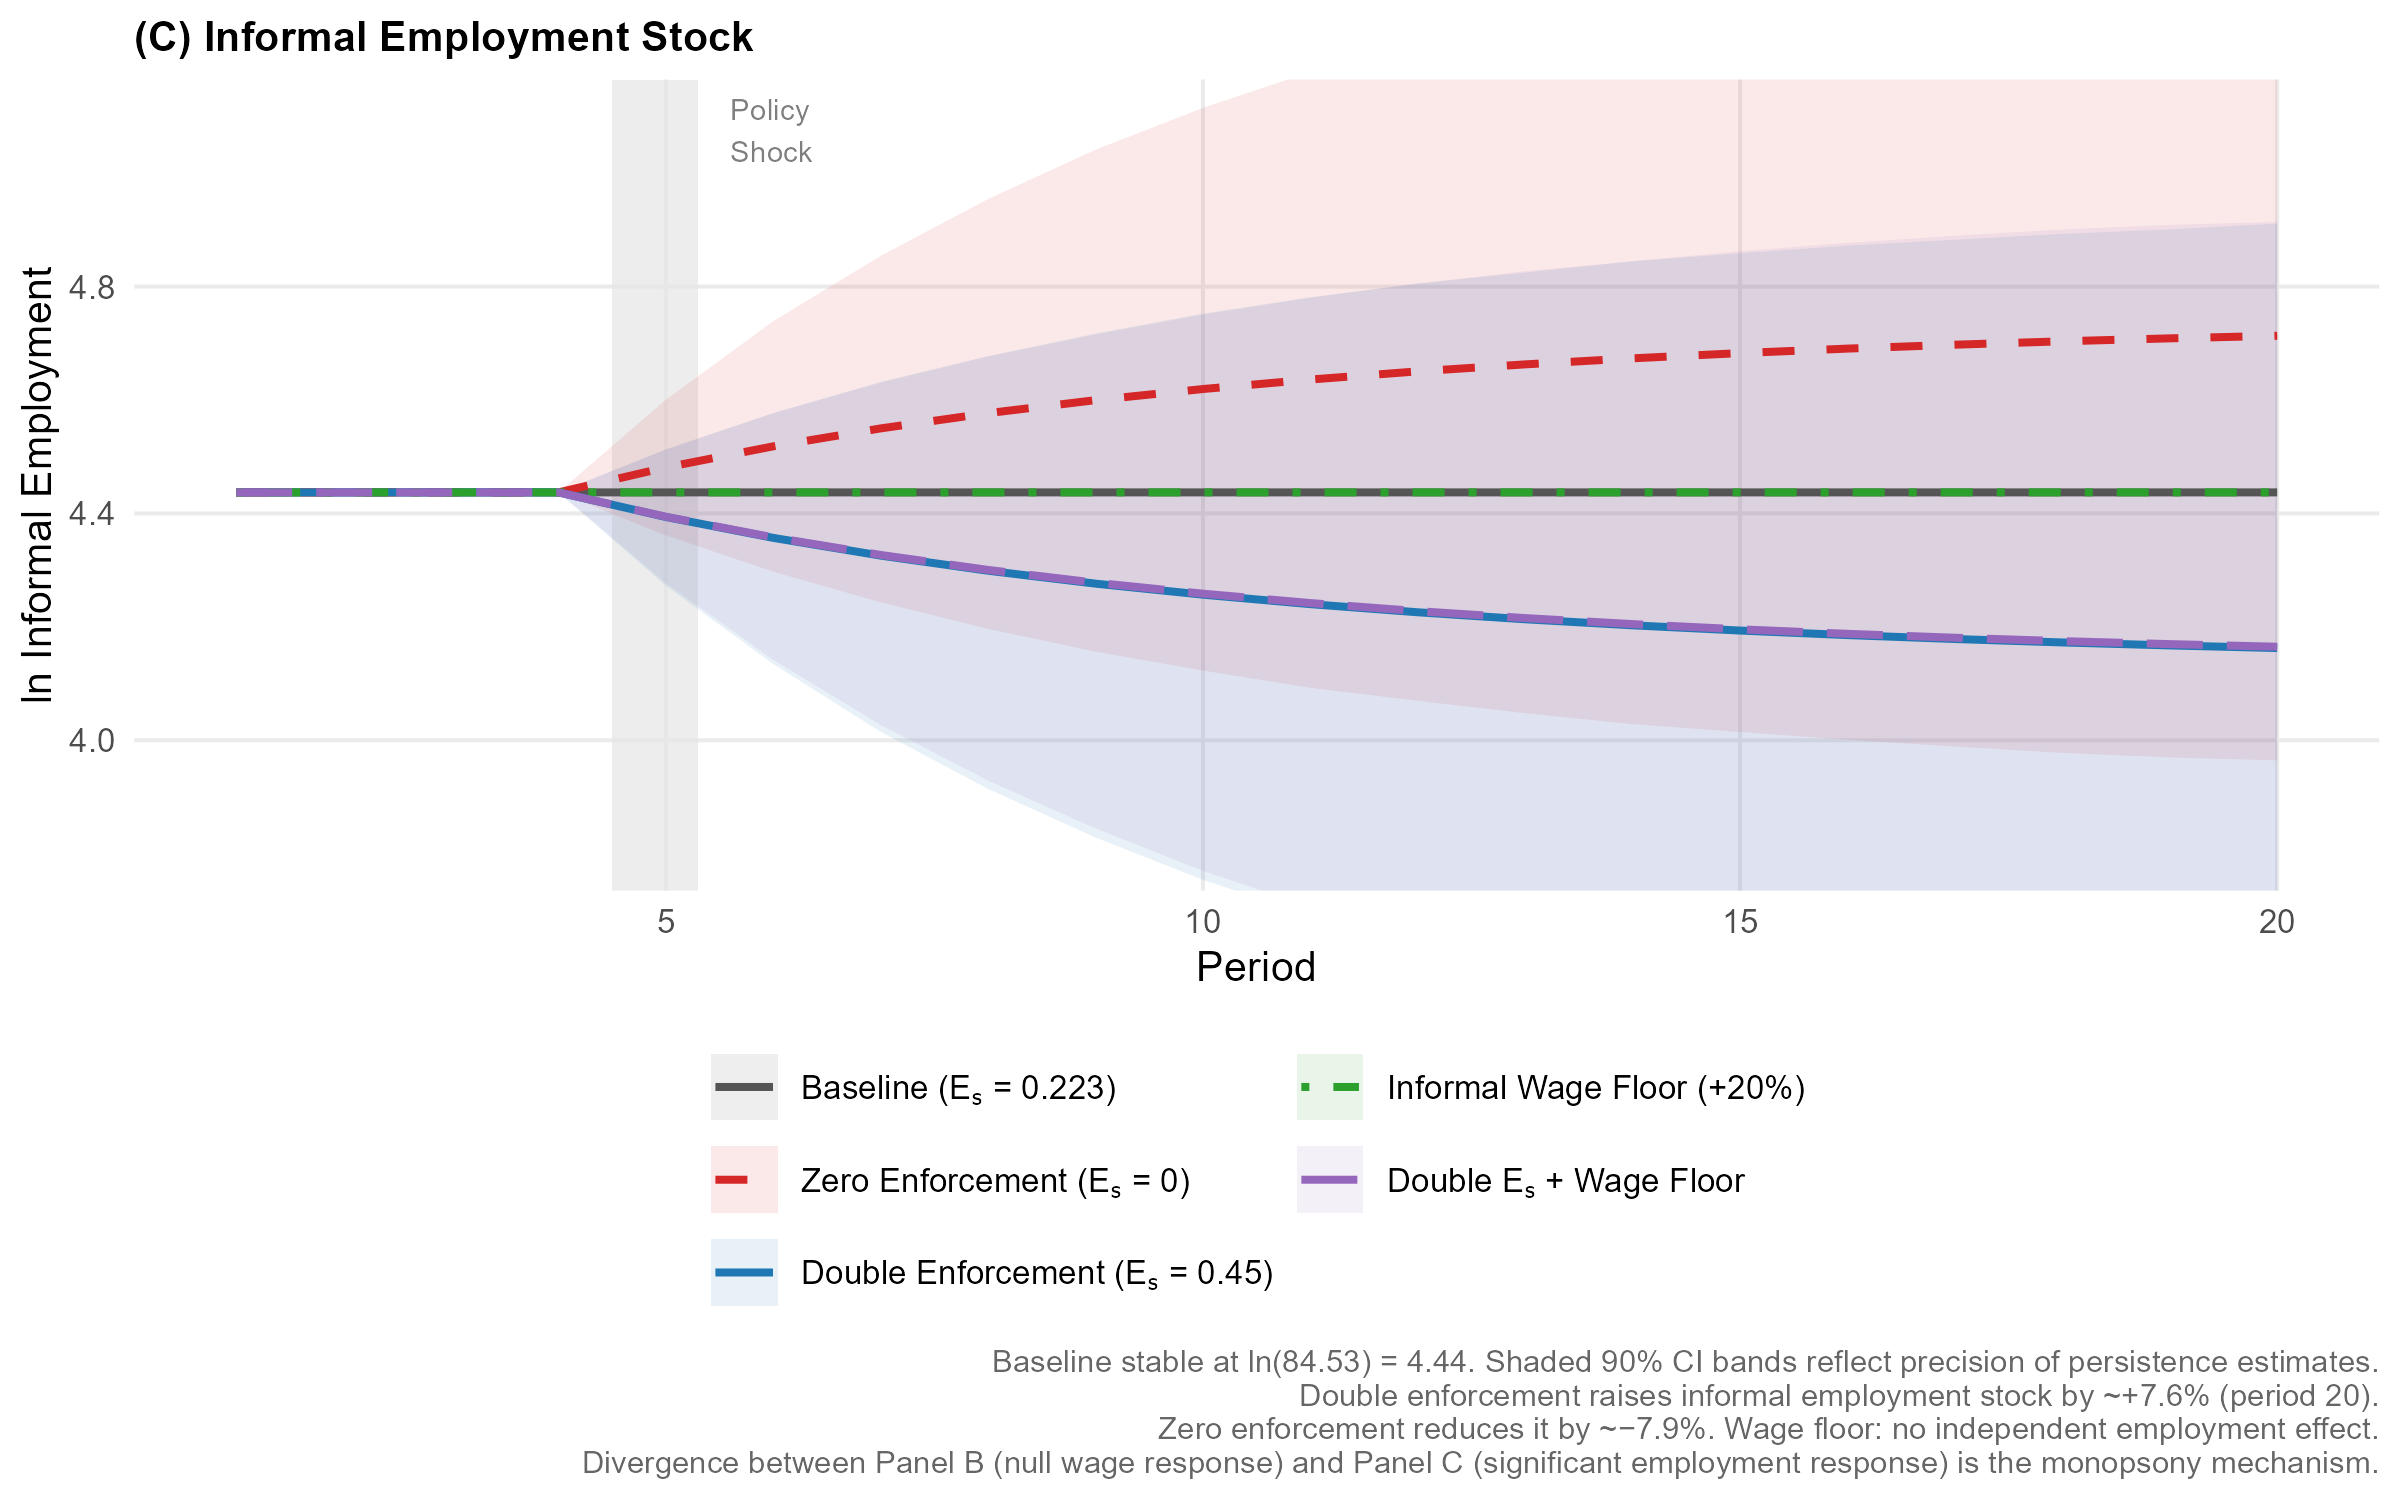
\includegraphics[width=0.65\textwidth]{../Output/images/figure_policy_sim_C_employment_v4}
  \caption{Simulation: Employment Impact}
  \label{fig:sim_emp}
\end{figure}



\textbf{Key Takeaways.} 
\begin{enumerate}[leftmargin=*]
  \item \textbf{Monopsony Persistence:} Increasing enforcement alone (Double Enforcement) reduced job counts but failed to raise wages.
  \item \textbf{The Wage Floor Solution:} Only a direct wage floor bypasses formal buyer power to sustainably raise informal earnings.
  \item \textbf{Inelastic Outsourcing:} Subcontracting remains a structural necessity of production, highly resilient to regulatory shocks.
\end{enumerate}

\section{Conclusion}
The evidence rejects the displacement hypothesis. India's textile value chains are characterized by \textbf{adverse incorporation}: formal firms modernization deepens, rather than dissolves, their reliance on precariously paid informal labor. Policy must pivot from policing factory gates to directly empowering the bargaining position of the informal base.

\bigskip
\noindent\rule{\textwidth}{0.4pt}
\vspace{4pt}
\noindent\small\textit{Analytical excerpt from Chapter 5 of the author's MA dissertation. Full references and methodology available on request.}
\end{document}
